\section{Alloy}

Here is displayed the fully commented alloy code used to model the portion of city
our system will interact with

\lstinputlisting[breaklines=true]{../../alloy/model.als}

\section{Generated world}

Diagram \ref{fig:generated_world} shows one of the instances generate by alloy, running the \textit{show} predicate

\begin{sidewaysfigure}
  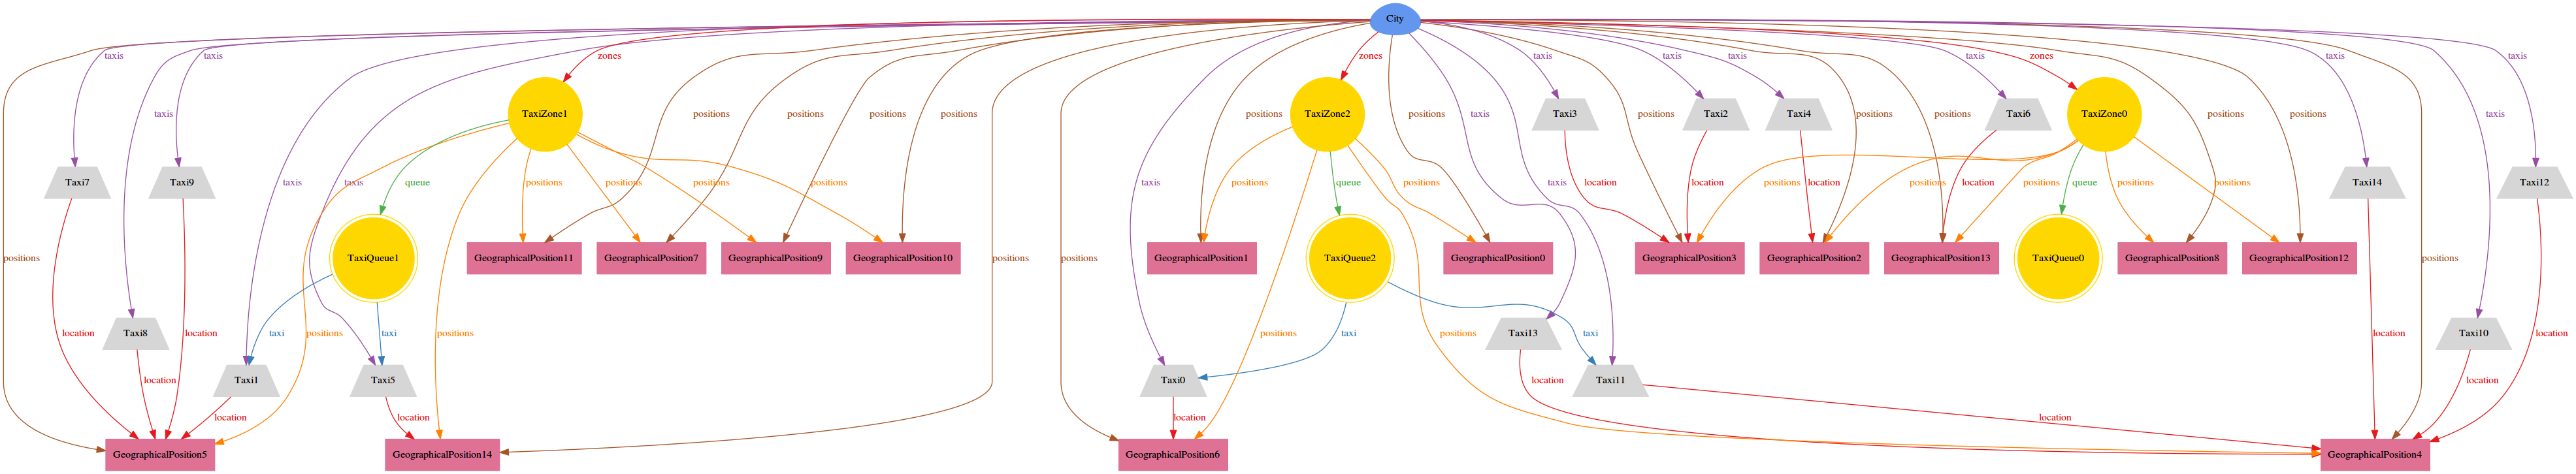
\includegraphics [scale=0.3]{../../alloy/generated_world.png}
  \caption{\label{fig:generated_world}}
\end{sidewaysfigure}

\section{Solver output}

\begin{lstlisting}
6 commands were executed. The results are:
  #1: .taxiMove is consistent.
  #2: .taxiIsUnavailable is consistent.
  #3: .taxiIsAvailable is consistent.
  #4: .taxiBecomeUnavailable is consistent.
  #5: .taxiBecomeAvailable is consistent.
  #6: .show is consistent.
\end{lstlisting}
